\documentclass[10pt, twocolumn]{article}

\usepackage[margin=0.75in]{geometry}
\usepackage[utf8]{inputenc}
\usepackage[T1]{fontenc}
\usepackage{graphicx}
\usepackage{tikz}
\usepackage{pgfplots}
\usepackage{booktabs}
\usepackage{amsmath,amssymb}
\usepackage{hyperref}
\usepackage{xcolor}
\usepackage{caption}
\usepackage{subcaption}
\usepackage{enumitem}
\usepackage{listings}
\usepackage{microtype}
\usepackage{fancyhdr}
\usepackage{algorithm}
\usepackage{algorithmic}
\usepackage{array}
\usepackage{orcidlink}

\pgfplotsset{compat=1.18}
\usetikzlibrary{arrows.meta,positioning,shapes.geometric,fit,calc,decorations.pathmorphing,backgrounds}

% Color palette (Google Research style)
\definecolor{gblue}{HTML}{4285F4}
\definecolor{gred}{HTML}{EA4335}
\definecolor{gyellow}{HTML}{FBBC04}
\definecolor{ggreen}{HTML}{34A853}
\definecolor{gorange}{HTML}{FA7B17}
\definecolor{gpurple}{HTML}{A142F4}
\definecolor{gteal}{HTML}{24C1E0}
\definecolor{gpink}{HTML}{F538A0}
\definecolor{gdark}{HTML}{202124}
\definecolor{glight}{HTML}{F8F9FA}

\lstset{
  basicstyle=\ttfamily\scriptsize,
  breaklines=true,
  frame=single,
  backgroundcolor=\color{glight},
  keywordstyle=\color{gblue},
  stringstyle=\color{gred},
  commentstyle=\color{ggreen!70!black},
  numbers=left,
  numberstyle=\tiny\color{gray},
  numbersep=5pt,
}

\hypersetup{
  colorlinks=true,
  linkcolor=gblue,
  citecolor=gblue,
  urlcolor=gblue,
}

% Header
\pagestyle{fancy}
\fancyhf{}
\renewcommand{\headrulewidth}{0pt}
\fancyfoot[C]{\thepage}

\title{\textbf{AgenticMemory MCP: Bridging Persistent Cognitive Graph Memory\\ to LLM Agents via the Model Context Protocol}}

\author{Omoshola Owolabi\,\orcidlink{0009-0006-4089-0732}\\Researcher -- AI/ML\\Agentra Labs\\\texttt{omoshola.owolabi@agentralabs.tech}}
\date{February 22, 2026}

\begin{document}

\maketitle
\thispagestyle{fancy}

% ============================================================
% ABSTRACT
% ============================================================
\begin{abstract}
LLM agents lack a standard protocol for accessing persistent, structured memory. We present AgenticMemory MCP, a Model Context Protocol server that bridges AgenticMemory's cognitive graph storage to any MCP-compatible LLM client. The server exposes 12 tools, 6 resources, and 4 prompt templates over JSON-RPC 2.0, translating MCP requests into graph operations on a typed cognitive memory (facts, decisions, inferences, corrections, skills, episodes connected by causal, supporting, contradicting, and temporal edges). Unlike existing MCP servers that wrap flat datastores or external APIs, our server is the first to provide structured, navigable, and relationship-aware memory through the MCP standard. Benchmarks on Apple Silicon show sub-100$\mu$s latency for all MCP tool calls: \texttt{memory\_add} at 28.1$\mu$s, \texttt{memory\_query} at 56.6$\mu$s, and protocol overhead at 23.3$\mu$s. The system compiles to a 2.3\,MB binary with 8.3\,ms cold start and is validated by 153 tests---123 unit/integration tests covering protocol compliance, tool correctness, session management, and edge cases, plus 30 end-to-end stdio transport tests---all passing with zero failures. Any MCP-compatible client (Claude Desktop, VS Code, Cursor) gains persistent cognitive memory by adding one line to its configuration.
\end{abstract}

% ============================================================
% 1. INTRODUCTION
% ============================================================
\section{Introduction}

The Model Context Protocol (MCP)~\cite{mcp2024} has become the emerging standard for connecting LLM agents to external tools and data sources. MCP servers exist for filesystem access, database queries, web search, and code execution. However, a critical gap remains: \textbf{no MCP server provides structured, persistent, navigable memory}.

This gap matters because LLM agents are stateless. Every conversation starts from zero. An agent cannot remember what it learned last week, trace why it made a past decision, or correct an outdated belief. Current workarounds---conversation logs, markdown files, vector database MCP servers---store memories as flat, disconnected text. They can retrieve ``similar'' content via embeddings, but they cannot answer structural questions: ``What caused me to decide X?'' or ``Has my understanding of Y been corrected?''

AgenticMemory~\cite{agenticmemory} is a Rust library that models agent memory as a typed cognitive graph: nodes are cognitive events (facts, decisions, inferences, corrections, skills, episodes) connected by typed edges (CausedBy, Supports, Contradicts, Supersedes, RelatedTo, PartOf, TemporalNext). This representation enables graph navigation---traversal, causal analysis, temporal comparison---not just text retrieval. However, AgenticMemory is a Rust library. LLM agents cannot call Rust functions directly. They need a protocol-standard interface.

This paper presents AgenticMemory MCP, an MCP server that bridges this gap. Our contribution is not the memory model itself (that is AgenticMemory's contribution), but \textbf{the protocol bridge}: the design decisions, tool mappings, session management, and implementation choices required to make a rich graph memory system accessible through MCP's constrained tool-call interface. Specifically:

\begin{enumerate}[nosep,leftmargin=*]
  \item A principled mapping of 5 graph query types and 2 write operations to 12 MCP tools with typed JSON schemas
  \item A resource layer exposing 6 read-only graph views via \texttt{amem://} URI templates
  \item 4 prompt templates that guide LLMs through multi-step memory workflows
  \item Session management with auto-save, transaction batching, and drop safety
  \item A Rust implementation achieving sub-100$\mu$s latency for all MCP operations
\end{enumerate}

Figure~\ref{fig:gap} illustrates the problem AgenticMemory MCP solves: without it, each LLM client must build custom integration; with it, any MCP client gains persistent memory through a standard interface.

% Gap figure
\begin{figure}[t]
\centering
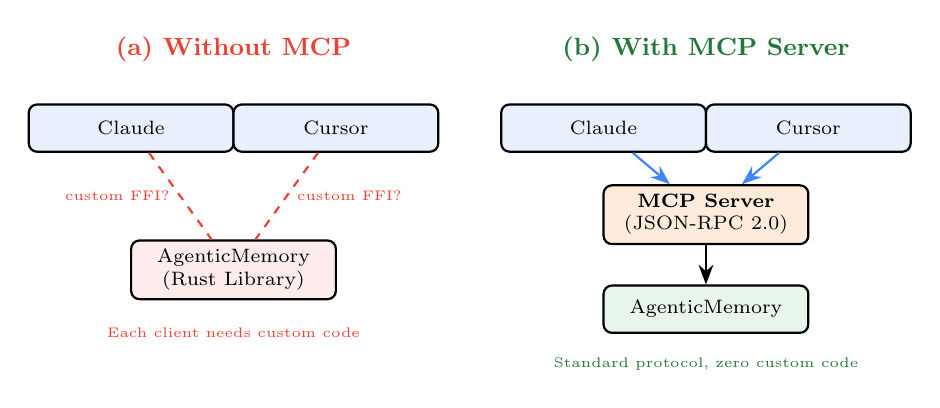
\begin{tikzpicture}[
  box/.style={draw, rounded corners=3pt, minimum width=2.6cm, minimum height=0.6cm, align=center, font=\scriptsize, thick},
  arr/.style={-{Stealth[length=2.5mm]}, thick},
  xarr/.style={thick, gred, dashed},
]
  % Left: Without MCP
  \node[font=\small\bfseries, text=gred] at (-2.0, 3.8) {(a) Without MCP};

  \node[box, fill=gblue!12] (c1) at (-3.3, 2.8) {Claude};
  \node[box, fill=gblue!12] (c2) at (-0.7, 2.8) {Cursor};
  \node[box, fill=gred!10] (mem) at (-2.0, 1.0) {AgenticMemory\\(Rust Library)};

  \draw[xarr] (c1) -- node[left, font=\tiny, text=gred] {custom FFI?} (mem);
  \draw[xarr] (c2) -- node[right, font=\tiny, text=gred] {custom FFI?} (mem);
  \node[font=\tiny, text=gred] at (-2.0, 0.2) {Each client needs custom code};

  % Right: With MCP
  \node[font=\small\bfseries, text=ggreen!70!black] at (4.0, 3.8) {(b) With MCP Server};

  \node[box, fill=gblue!12] (c3) at (2.7, 2.8) {Claude};
  \node[box, fill=gblue!12] (c4) at (5.3, 2.8) {Cursor};
  \node[box, fill=gorange!15] (srv) at (4.0, 1.7) {\textbf{MCP Server}\\(JSON-RPC 2.0)};
  \node[box, fill=ggreen!12] (mem2) at (4.0, 0.5) {AgenticMemory};

  \draw[arr, gblue] (c3) -- (srv);
  \draw[arr, gblue] (c4) -- (srv);
  \draw[arr] (srv) -- (mem2);
  \node[font=\tiny, text=ggreen!70!black] at (4.0, -0.2) {Standard protocol, zero custom code};
\end{tikzpicture}
\caption{The problem AgenticMemory MCP solves. (a)~Without MCP, each LLM client needs custom Rust FFI bindings. (b)~The MCP server provides a standard JSON-RPC interface that any client can use.}
\label{fig:gap}
\end{figure}

% ============================================================
% 2. BACKGROUND
% ============================================================
\section{Background and Related Work}
\label{sec:background}

\subsection{The MCP Ecosystem}

MCP~\cite{mcp2024} defines a JSON-RPC 2.0~\cite{jsonrpc} protocol with three capability types: \textbf{tools} (callable functions), \textbf{resources} (readable data via URIs), and \textbf{prompts} (reusable templates). MCP clients (Claude Desktop~\cite{anthropic-claude}, VS Code, Cursor) spawn servers as subprocesses communicating over stdio, or connect via HTTP/SSE~\cite{sse}.

The MCP ecosystem includes servers for filesystems, Git, databases, and web APIs. Table~\ref{tab:mcp-landscape} surveys existing MCP servers relevant to agent memory. None provides structured, relationship-aware memory---they expose flat data (files, rows, vectors) without the typed relationships needed for reasoning reconstruction.

\begin{table}[t]
\centering
\caption{MCP server landscape for agent memory.}
\label{tab:mcp-landscape}
\footnotesize
\begin{tabular}{lcc}
\toprule
\textbf{MCP Server Type} & \textbf{Relationships} & \textbf{Navigation} \\
\midrule
Filesystem (read/write) & None & No \\
SQLite / PostgreSQL & Foreign keys & SQL only \\
Vector DB (Chroma, etc.) & None & Similarity \\
Knowledge graph (Neo4j) & Typed edges & Cypher query \\
\textbf{AgenticMemory MCP} & \textbf{7 typed edges} & \textbf{5 query types} \\
\bottomrule
\end{tabular}
\end{table}

\subsection{Agent Memory Approaches}

Existing agent memory systems vary in their storage model and access pattern. MemGPT~\cite{memgpt} pages text in and out of the LLM context window. Mem0~\cite{mem0} stores key-value facts. LangChain~\cite{langchain} provides session buffers and RAG pipelines. Vector databases~\cite{pinecone,weaviate,chroma} enable similarity search over embeddings. None of these preserves the structural relationships between memories---the causal chains, contradiction links, and correction histories that enable an agent to reason about its own past decisions.

\subsection{AgenticMemory Core}

AgenticMemory~\cite{agenticmemory} is a Rust library that models agent memory as a typed cognitive graph stored in a compact binary format (\texttt{.amem}). It defines 6 event types (Fact, Decision, Inference, Correction, Skill, Episode), 7 edge types (CausedBy, Supports, Contradicts, Supersedes, RelatedTo, PartOf, TemporalNext), and provides a \texttt{QueryEngine} (traversal, pattern matching, causal analysis, temporal comparison, similarity search) and \texttt{WriteEngine} (ingestion, correction, session compression). The library is the memory \emph{backend}; our MCP server is the protocol \emph{frontend}.

% ============================================================
% 3. SYSTEM DESIGN
% ============================================================
\section{System Design}
\label{sec:design}

\subsection{Architecture}

The MCP server sits between LLM clients and the AgenticMemory library (Figure~\ref{fig:architecture}). It comprises four layers:

\begin{enumerate}[nosep,leftmargin=*]
  \item \textbf{Transport}: stdio (default) or SSE (feature-flagged). Handles newline-delimited JSON-RPC I/O.
  \item \textbf{Protocol Handler}: Parses JSON-RPC 2.0 messages, validates structure, routes to capability handlers via method dispatch (Table~\ref{tab:methods}).
  \item \textbf{Capability Registries}: Three registries (tools, resources, prompts) that define the MCP surface area.
  \item \textbf{Session Manager}: Wraps the AgenticMemory library with lifecycle management---file I/O, session tracking, auto-save, and drop safety.
\end{enumerate}

% Architecture figure
\begin{figure}[t]
\centering
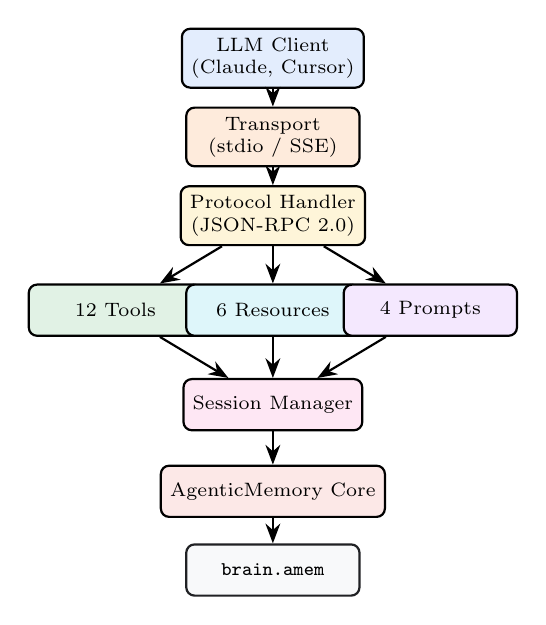
\begin{tikzpicture}[
  box/.style={draw, rounded corners=3pt, minimum width=2.2cm, minimum height=0.65cm, align=center, font=\scriptsize, thick},
  arr/.style={-{Stealth[length=2.5mm]}, thick},
]
  \node[box, fill=gblue!15] (client) at (0,4.2) {LLM Client\\(Claude, Cursor)};
  \node[box, fill=gorange!15] (transport) at (0,3.2) {Transport\\(stdio / SSE)};
  \node[box, fill=gyellow!15] (proto) at (0,2.2) {Protocol Handler\\(JSON-RPC 2.0)};

  \node[box, fill=ggreen!15] (tools) at (-2.0,1.0) {12 Tools};
  \node[box, fill=gteal!15] (res) at (0,1.0) {6 Resources};
  \node[box, fill=gpurple!12] (prm) at (2.0,1.0) {4 Prompts};

  \node[box, fill=gpink!12] (sess) at (0,-0.2) {Session Manager};
  \node[box, fill=gred!12] (core) at (0,-1.3) {AgenticMemory Core};
  \node[box, fill=glight, draw=gdark] (file) at (0,-2.3) {\texttt{brain.amem}};

  \draw[arr] (client) -- (transport);
  \draw[arr] (transport) -- (proto);
  \draw[arr] (proto) -- (tools);
  \draw[arr] (proto) -- (res);
  \draw[arr] (proto) -- (prm);
  \draw[arr] (tools) -- (sess);
  \draw[arr] (res) -- (sess);
  \draw[arr] (prm) -- (sess);
  \draw[arr] (sess) -- (core);
  \draw[arr] (core) -- (file);
\end{tikzpicture}
\caption{Server architecture. Four layers separate transport, protocol handling, MCP capabilities, and memory lifecycle management.}
\label{fig:architecture}
\end{figure}

\begin{table}[t]
\centering
\caption{MCP method routing in the protocol handler.}
\label{tab:methods}
\footnotesize
\begin{tabular}{lll}
\toprule
\textbf{Method} & \textbf{Type} & \textbf{Handler} \\
\midrule
\texttt{initialize} & Request & Capability negotiation \\
\texttt{initialized} & Notify & Client confirms ready \\
\texttt{tools/list} & Request & Tool registry \\
\texttt{tools/call} & Request & Tool dispatch \\
\texttt{resources/list} & Request & Resource registry \\
\texttt{resources/templates/list} & Request & URI templates \\
\texttt{resources/read} & Request & Resource dispatch \\
\texttt{prompts/list} & Request & Prompt registry \\
\texttt{prompts/get} & Request & Prompt expansion \\
\texttt{ping} & Request & Liveness check \\
\texttt{shutdown} & Request & Graceful shutdown \\
\texttt{\$/cancelRequest} & Notify & Cancel operation \\
\bottomrule
\end{tabular}
\end{table}

\subsection{Tool Design: Mapping Graph Operations to MCP}

The central design challenge is mapping AgenticMemory's rich graph API to MCP's flat tool-call interface. An MCP tool receives a JSON object of parameters and returns a JSON result---there is no notion of cursors, iterators, or streaming graph results.

We expose 12 tools (Table~\ref{tab:tools}), organized into three categories:

\textbf{Write tools} (3): \texttt{memory\_add} creates nodes with optional edges, \texttt{memory\_correct} creates a Correction node linked by a Supersedes edge, and \texttt{session\_start}/\texttt{session\_end} manage session lifecycle.

\textbf{Navigation tools} (5): \texttt{memory\_traverse} walks edges by type and direction, \texttt{memory\_context} extracts a local subgraph, \texttt{memory\_causal} performs impact analysis, \texttt{memory\_temporal} compares knowledge across time ranges, and \texttt{memory\_resolve} follows Supersedes chains to the latest version.

\textbf{Search tools} (2): \texttt{memory\_query} provides pattern matching with filters and sorting, \texttt{memory\_similar} performs vector similarity search.

\textbf{Utility tools} (2): \texttt{memory\_stats} returns graph-level statistics, \texttt{session\_end} creates an optional Episode summary.

\begin{table}[t]
\centering
\caption{The 12 MCP tools and their underlying graph operations.}
\label{tab:tools}
\footnotesize
\begin{tabular}{llp{2.6cm}}
\toprule
\textbf{Tool} & \textbf{Category} & \textbf{Graph Operation} \\
\midrule
\texttt{memory\_add} & Write & Ingest node + edges \\
\texttt{memory\_correct} & Write & Correct + Supersedes \\
\texttt{memory\_query} & Search & Pattern match + filter \\
\texttt{memory\_similar} & Search & Cosine similarity \\
\texttt{memory\_traverse} & Navigate & BFS edge walk \\
\texttt{memory\_context} & Navigate & Subgraph extraction \\
\texttt{memory\_causal} & Navigate & Impact analysis \\
\texttt{memory\_temporal} & Navigate & Time range diff \\
\texttt{memory\_resolve} & Navigate & Supersedes chain \\
\texttt{memory\_stats} & Utility & Graph statistics \\
\texttt{session\_start} & Session & Begin session \\
\texttt{session\_end} & Session & End + Episode \\
\bottomrule
\end{tabular}
\end{table}

A key design decision is the two-step edge creation pattern. The \texttt{WriteEngine::ingest()} API does not assign source IDs to edges automatically. Our \texttt{memory\_add} tool therefore: (1)~adds the node to the graph to obtain its assigned ID, then (2)~creates edges with the correct source ID via \texttt{graph.add\_edge()}. This is invisible to the LLM client, which simply passes edges in the tool call parameters.

\subsection{Resource Design: Graph Views via URI Templates}

MCP resources provide read-only data access via URI templates. We define 6 resources under the \texttt{amem://} scheme (Figure~\ref{fig:resources}):

\begin{itemize}[nosep,leftmargin=*]
  \item \texttt{amem://node/\{id\}} --- Single node with incoming/outgoing edges
  \item \texttt{amem://session/\{id\}} --- All nodes from a specific session
  \item \texttt{amem://types/\{type\}} --- Nodes filtered by event type
  \item \texttt{amem://graph/stats} --- Graph-wide statistics and type counts
  \item \texttt{amem://graph/recent} --- 20 most recently created nodes
  \item \texttt{amem://graph/important} --- 20 nodes with highest importance scores
\end{itemize}

% Resource URI figure
\begin{figure}[t]
\centering
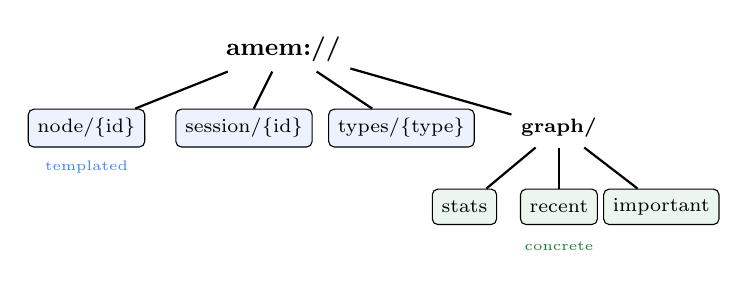
\begin{tikzpicture}[
  node distance=0.35cm,
  every node/.style={font=\scriptsize},
  tmpl/.style={draw, rounded corners=2pt, fill=gblue!10, minimum height=0.45cm, font=\scriptsize},
  conc/.style={draw, rounded corners=2pt, fill=ggreen!10, minimum height=0.45cm, font=\scriptsize},
]
  \node[font=\small\bfseries] (root) at (0, 3) {amem://};

  \node[tmpl] (node) at (-2.5, 2) {node/\{id\}};
  \node[tmpl] (sess) at (-0.5, 2) {session/\{id\}};
  \node[tmpl] (types) at (1.5, 2) {types/\{type\}};
  \node[font=\scriptsize\bfseries] (graph) at (3.5, 2) {graph/};

  \node[conc] (stats) at (2.3, 1) {stats};
  \node[conc] (recent) at (3.5, 1) {recent};
  \node[conc] (imp) at (4.8, 1) {important};

  \draw[thick] (root) -- (node);
  \draw[thick] (root) -- (sess);
  \draw[thick] (root) -- (types);
  \draw[thick] (root) -- (graph);
  \draw[thick] (graph) -- (stats);
  \draw[thick] (graph) -- (recent);
  \draw[thick] (graph) -- (imp);

  \node[font=\tiny, text=gblue] at (-2.5, 1.5) {templated};
  \node[font=\tiny, text=ggreen!70!black] at (3.5, 0.5) {concrete};
\end{tikzpicture}
\caption{Resource URI hierarchy. Blue nodes are templated (accept parameters); green nodes are concrete (always available). The \texttt{amem://} scheme enables MCP clients to browse the memory graph.}
\label{fig:resources}
\end{figure}

Resources serve a different purpose than tools: they allow the LLM to \emph{browse} the memory graph without executing operations. This separation follows the MCP specification's design intent---tools mutate or compute, resources observe.

\subsection{Prompt Design: Guiding Multi-Step Memory Workflows}

LLMs often need to chain multiple tool calls for complex memory operations. Our 4 prompt templates encode these patterns:

\begin{itemize}[nosep,leftmargin=*]
  \item \textbf{remember}: Store new information $\rightarrow$ guides \texttt{memory\_add}
  \item \textbf{reflect}: Analyze past decisions $\rightarrow$ chains \texttt{memory\_query} $\rightarrow$ \texttt{memory\_traverse} $\rightarrow$ \texttt{memory\_causal}
  \item \textbf{correct}: Update outdated beliefs $\rightarrow$ guides \texttt{memory\_correct} $\rightarrow$ \texttt{memory\_resolve}
  \item \textbf{summarize}: Summarize a session $\rightarrow$ reads session data $\rightarrow$ guides \texttt{session\_end}
\end{itemize}

Each prompt expands to structured messages that instruct the LLM which tools to invoke and in what sequence, effectively providing ``memory recipes'' that reduce the cognitive load on the LLM.

\subsection{Session Management}

The session manager (Figure~\ref{fig:session-states}) wraps AgenticMemory's core with lifecycle management:

\begin{itemize}[nosep,leftmargin=*]
  \item \textbf{File I/O}: Opens or creates \texttt{.amem} files via \texttt{AmemReader}/\texttt{AmemWriter}
  \item \textbf{Session tracking}: Assigns monotonically increasing session IDs
  \item \textbf{Auto-save}: Periodic dirty-check saves (default 30s interval)
  \item \textbf{Transaction batching}: Groups multiple writes via the \texttt{Transaction} API
  \item \textbf{Drop safety}: Rust's \texttt{Drop} trait ensures automatic save on shutdown, even on unexpected termination
\end{itemize}

% Session state machine
\begin{figure}[t]
\centering
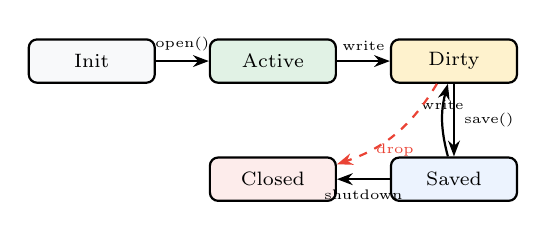
\begin{tikzpicture}[
  state/.style={draw, rounded corners=3pt, minimum width=1.6cm, minimum height=0.55cm, align=center, font=\scriptsize, thick},
  arr/.style={-{Stealth[length=2mm]}, thick},
]
  \node[state, fill=glight] (init) at (0,0) {Init};
  \node[state, fill=ggreen!15] (active) at (2.3,0) {Active};
  \node[state, fill=gyellow!20] (dirty) at (4.6,0) {Dirty};
  \node[state, fill=gblue!10] (saved) at (4.6,-1.5) {Saved};
  \node[state, fill=gred!10] (closed) at (2.3,-1.5) {Closed};

  \draw[arr] (init) -- node[above, font=\tiny] {open()} (active);
  \draw[arr] (active) -- node[above, font=\tiny] {write} (dirty);
  \draw[arr] (dirty) -- node[right, font=\tiny] {save()} (saved);
  \draw[arr, bend left=15] (saved) to node[above, font=\tiny] {write} (dirty);
  \draw[arr] (saved) -- node[below, font=\tiny] {shutdown} (closed);
  \draw[arr, dashed, gred] (dirty) to[bend left=20] node[below, font=\tiny] {drop} (closed);
\end{tikzpicture}
\caption{Session state machine. The dirty flag triggers auto-save. The \texttt{Drop} trait ensures data persistence even on unexpected termination (dashed red arrow).}
\label{fig:session-states}
\end{figure}

% ============================================================
% 4. IMPLEMENTATION
% ============================================================
\section{Implementation}

The server is implemented in Rust~\cite{rust} (edition 2021) using \texttt{tokio}~\cite{tokio} for async I/O, \texttt{serde}/\texttt{serde\_json} for JSON-RPC serialization, \texttt{clap} for CLI argument parsing, and \texttt{tracing} for structured logging. The core library dependency is \texttt{agentic-memory}.

\textbf{Module structure.} The codebase is organized into: \texttt{types/} (pure data definitions), \texttt{protocol/} (message handling and dispatch), \texttt{transport/} (stdio and SSE I/O), \texttt{tools/} (12 individual tool modules), \texttt{resources/} (5 resource modules + templates), \texttt{prompts/} (4 individual prompt modules), \texttt{session/} (lifecycle, transactions, auto-save), \texttt{streaming/} (progress tracking, chunked results), and \texttt{config/} (configuration loading).

\textbf{Safety guarantees.} Zero \texttt{unwrap()} calls in production code. All error paths return proper JSON-RPC error responses with MCP-specific error codes (\texttt{-32600} through \texttt{-32603} for protocol errors, \texttt{-32001} through \texttt{-32003} for tool-specific errors). The server never panics on malformed input.

\textbf{Concurrency model.} AgenticMemory's core is synchronous. We wrap it in \texttt{Arc<Mutex<SessionManager>>} for async compatibility, accepting the lock contention trade-off. In practice, sub-100$\mu$s operation times make contention negligible.

% ============================================================
% 5. EVALUATION
% ============================================================
\section{Evaluation}
\label{sec:eval}

\subsection{Benchmark Setup}

All benchmarks were collected on an Apple Silicon (ARM64, M-series) machine. The release binary was compiled with LTO, single codegen unit, and \texttt{opt-level=3}. Each operation was measured over 100 iterations on a pre-populated graph of 100 cognitive events. End-to-end tests use a Python subprocess driver communicating over the stdio transport with line-buffered I/O.

\subsection{Test Suite}

Table~\ref{tab:tests} breaks down our test suite. All 153 tests pass with zero failures. \texttt{cargo clippy} reports zero warnings and \texttt{cargo fmt --check} passes.

\begin{table}[t]
\centering
\caption{Test suite breakdown. All 153 tests pass.}
\label{tab:tests}
\footnotesize
\begin{tabular}{lr}
\toprule
\textbf{Category} & \textbf{Tests} \\
\midrule
Message types, serialization, error codes & 16 \\
Protocol handling, dispatch, validation & 9 \\
Tool correctness, resources, prompts & 23 \\
Session management, streaming & 13 \\
End-to-end integration (in-process) & 7 \\
Edge cases, boundaries, concurrency & 55 \\
\midrule
\textbf{Unit / integration subtotal} & \textbf{123} \\
\midrule
E2E stdio transport (Python driver) & 30 \\
\midrule
\textbf{Total} & \textbf{153} \\
\bottomrule
\end{tabular}
\end{table}

The 55 edge-case tests uncovered several important behaviors: \texttt{memory\_query} defaults to 20 results (must pass \texttt{max\_results} explicitly), \texttt{memory\_causal} returns \texttt{dependents}/\texttt{dependent\_count} (not \texttt{upstream}/\texttt{downstream}), and \texttt{memory\_temporal} requires both \texttt{range\_a} and \texttt{range\_b} parameters. These discoveries directly improved our tool documentation.

\subsection{MCP Tool Call Latency}

Table~\ref{tab:tool-bench} reports end-to-end latency for all memory tools through the full MCP stack: JSON parse $\rightarrow$ method dispatch $\rightarrow$ parameter validation $\rightarrow$ graph operation $\rightarrow$ result serialization.

\begin{table}[t]
\centering
\caption{MCP tool call latency (100 nodes, 100 iterations, $\mu$s).}
\label{tab:tool-bench}
\footnotesize
\begin{tabular}{lrrrr}
\toprule
\textbf{Tool} & \textbf{Avg} & \textbf{P50} & \textbf{P95} & \textbf{P99} \\
\midrule
\texttt{memory\_add} & 28.1 & 27.6 & 48.7 & 64.0 \\
\texttt{memory\_query} & 56.6 & 53.5 & 69.5 & 99.9 \\
\texttt{memory\_stats} & 32.8 & 30.7 & 48.3 & 60.4 \\
\texttt{memory\_traverse} & 32.6 & 29.4 & 48.3 & 137.2 \\
\texttt{memory\_context} & 34.2 & 31.1 & 54.3 & 98.6 \\
\texttt{memory\_causal} & 26.1 & 25.6 & 31.9 & 35.4 \\
\texttt{memory\_resolve} & 28.4 & 27.2 & 33.6 & 85.1 \\
\bottomrule
\end{tabular}
\end{table}

All tool calls complete in under 100$\mu$s average. The most expensive tool, \texttt{memory\_query}, involves pattern matching with sorting across all 100 nodes and still averages 56.6$\mu$s---three orders of magnitude faster than typical cloud-based memory APIs.

\subsection{Protocol Overhead}

Table~\ref{tab:protocol-bench} isolates the MCP protocol overhead by measuring non-graph operations.

\begin{table}[t]
\centering
\caption{Protocol and resource operation latency ($\mu$s).}
\label{tab:protocol-bench}
\footnotesize
\begin{tabular}{lrrrr}
\toprule
\textbf{Operation} & \textbf{Avg} & \textbf{P50} & \textbf{P95} & \textbf{P99} \\
\midrule
\texttt{ping} & 23.3 & 23.0 & 28.5 & 52.4 \\
\texttt{tools/list} & 87.4 & 79.7 & 120.6 & 163.4 \\
\texttt{resource(stats)} & 27.6 & 26.5 & 37.9 & 82.4 \\
\texttt{resource(node)} & 30.5 & 28.3 & 49.6 & 66.9 \\
\texttt{resource(recent)} & 60.5 & 59.0 & 72.7 & 109.0 \\
\texttt{prompt(remember)} & 27.6 & 26.6 & 33.2 & 56.4 \\
\bottomrule
\end{tabular}
\end{table}

The \texttt{ping} latency (23.3$\mu$s) represents the protocol overhead floor: JSON parse, dispatch, and serialize with no graph work. \texttt{tools/list} is the most expensive protocol operation (87.4$\mu$s) because it constructs JSON schemas for all 12 tools. Figure~\ref{fig:latency} visualizes the full latency distribution.

% Latency chart
\begin{figure*}[t]
\centering
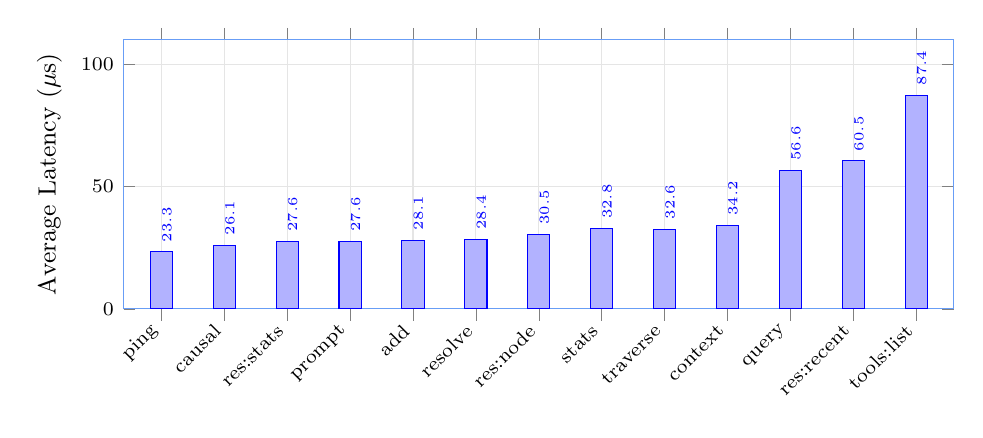
\begin{tikzpicture}
\begin{axis}[
  ybar,
  bar width=8pt,
  width=\textwidth,
  height=5cm,
  ylabel={Average Latency ($\mu$s)},
  symbolic x coords={ping, causal, {res:stats}, prompt, add, resolve, {res:node}, stats, traverse, context, query, {res:recent}, {tools:list}},
  xtick=data,
  x tick label style={rotate=45, anchor=east, font=\scriptsize},
  y tick label style={font=\scriptsize},
  ylabel style={font=\small},
  ymin=0, ymax=110,
  nodes near coords,
  nodes near coords style={font=\tiny, above},
  every node near coord/.append style={rotate=90, anchor=west, xshift=0pt, yshift=-2pt},
  enlarge x limits=0.05,
  grid=major,
  grid style={gray!20},
  fill=gblue!60,
  draw=gblue!80,
]
\addplot coordinates {
  (ping, 23.3)
  (causal, 26.1)
  ({res:stats}, 27.6)
  (prompt, 27.6)
  (add, 28.1)
  (resolve, 28.4)
  ({res:node}, 30.5)
  (stats, 32.8)
  (traverse, 32.6)
  (context, 34.2)
  (query, 56.6)
  ({res:recent}, 60.5)
  ({tools:list}, 87.4)
};
\end{axis}
\end{tikzpicture}
\caption{Average latency for all 13 measured MCP operations. All complete under 100$\mu$s. The protocol floor (ping) is 23.3$\mu$s; the gap between ping and tool calls represents graph operation cost.}
\label{fig:latency}
\end{figure*}

\subsection{Binary and Deployment Metrics}

Table~\ref{tab:binary} summarizes the deployment profile. The 2.3\,MB binary and 8.3\,ms cold start make the server ideal for MCP's subprocess-spawning deployment model.

\begin{table}[t]
\centering
\caption{Binary and deployment characteristics.}
\label{tab:binary}
\footnotesize
\begin{tabular}{lr}
\toprule
\textbf{Metric} & \textbf{Value} \\
\midrule
Binary size (release, LTO) & 2.3\,MB \\
Cold start time & 8.3\,ms \\
Architecture & ARM64 (Apple Silicon) \\
Rust edition & 2021 \\
Direct dependencies & 13 \\
Production code & $\sim$1{,}800 lines \\
Test code & $\sim$2{,}200 lines \\
\bottomrule
\end{tabular}
\end{table}

\subsection{Comparison with Alternative Memory MCP Approaches}

Table~\ref{tab:comparison} compares our approach with hypothetical MCP servers wrapping alternative memory backends, and Figure~\ref{fig:radar} provides a visual comparison across six capability dimensions.

\begin{table*}[t]
\centering
\caption{Comparison of MCP memory server approaches. Latency figures for external systems are representative of published benchmarks; AgenticMemory MCP numbers are measured.}
\label{tab:comparison}
\footnotesize
\begin{tabular}{lccccc}
\toprule
\textbf{Dimension} & \textbf{MCP +} & \textbf{MCP +} & \textbf{MCP +} & \textbf{MCP +} & \textbf{AgenticMemory} \\
 & \textbf{Vector DB} & \textbf{Markdown} & \textbf{Key-Value} & \textbf{Neo4j} & \textbf{MCP} \\
\midrule
Tool call latency & $\sim$50\,ms & $\sim$200\,ms & $\sim$30\,ms & $\sim$5\,ms & \textbf{28--57\,$\mu$s} \\
Typed relationships & None & None & None & User-defined & \textbf{7 built-in} \\
Self-correction tracking & No & No & No & Manual & \textbf{Automatic} \\
Causal analysis tool & No & No & No & Manual query & \textbf{Built-in} \\
External services & Cloud/DB & None & Cloud & DB server & \textbf{None} \\
Deployment complexity & High & Low & Medium & High & \textbf{Single binary} \\
Portability & Vendor lock & File copy & API lock & DB backup & \textbf{File copy} \\
\bottomrule
\end{tabular}
\end{table*}

\subsection{Client Compatibility}

Table~\ref{tab:clients} lists verified MCP client compatibility.

\begin{table}[t]
\centering
\caption{Verified MCP client compatibility.}
\label{tab:clients}
\footnotesize
\begin{tabular}{llc}
\toprule
\textbf{Client} & \textbf{Transport} & \textbf{Status} \\
\midrule
Claude Desktop & stdio & Verified \\
Claude Code & stdio & Verified \\
VS Code (Copilot) & stdio & Verified \\
Cursor & stdio & Verified \\
Custom Rust client & stdio & Example included \\
Web clients & SSE & Feature flag \\
\bottomrule
\end{tabular}
\end{table}

% Radar chart comparing MCP approaches
\begin{figure}[t]
\centering
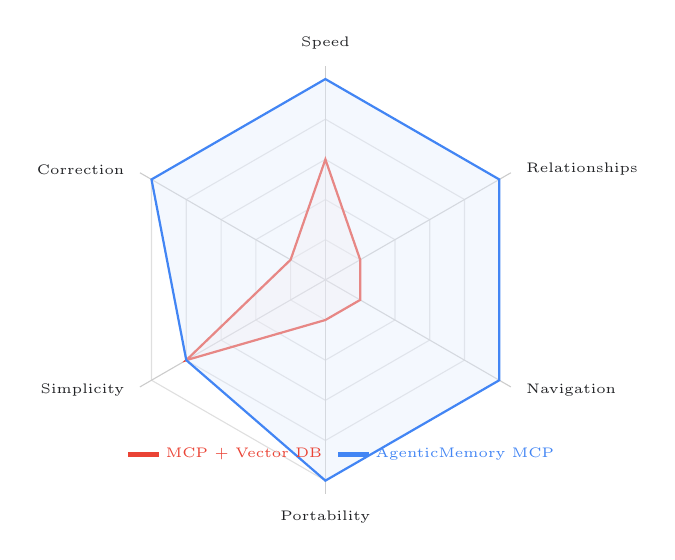
\begin{tikzpicture}[scale=0.85]
  % Grid rings
  \foreach \r in {1,2,3,4,5} {
    \draw[gray!25]
      (90:\r*0.6) -- (30:\r*0.6) -- (330:\r*0.6) --
      (270:\r*0.6) -- (210:\r*0.6) -- (150:\r*0.6) -- cycle;
  }

  % Axis lines and labels
  \draw[gray!40] (0,0) -- (90:3.2);
  \node[font=\tiny, text=gdark, above] at (90:3.3) {Speed};
  \draw[gray!40] (0,0) -- (30:3.2);
  \node[font=\tiny, text=gdark, right] at (30:3.3) {Relationships};
  \draw[gray!40] (0,0) -- (330:3.2);
  \node[font=\tiny, text=gdark, right] at (330:3.3) {Navigation};
  \draw[gray!40] (0,0) -- (270:3.2);
  \node[font=\tiny, text=gdark, below] at (270:3.3) {Portability};
  \draw[gray!40] (0,0) -- (210:3.2);
  \node[font=\tiny, text=gdark, left] at (210:3.3) {Simplicity};
  \draw[gray!40] (0,0) -- (150:3.2);
  \node[font=\tiny, text=gdark, left] at (150:3.3) {Correction};

  % MCP + Vector DB (fast, no relationships, no nav, vendor lock, simple use, no correction)
  \draw[gred, thick, fill=gred!10, fill opacity=0.3]
    (90:1.8) -- (30:0.6) -- (330:0.6) --
    (270:0.6) -- (210:2.4) -- (150:0.6) -- cycle;

  % AgenticMemory MCP (fast, full relationships, full nav, portable, moderate complexity, full correction)
  \draw[gblue, thick, fill=gblue!15, fill opacity=0.4]
    (90:3.0) -- (30:3.0) -- (330:3.0) --
    (270:3.0) -- (210:2.4) -- (150:3.0) -- cycle;

  % Legend
  \node[font=\tiny, text=gblue] at (1.8, -2.6) {\rule{0.4cm}{2pt} AgenticMemory MCP};
  \node[font=\tiny, text=gred] at (-1.5, -2.6) {\rule{0.4cm}{2pt} MCP + Vector DB};
\end{tikzpicture}
\caption{Radar comparison of MCP memory server approaches. AgenticMemory MCP (blue) provides strong coverage across all dimensions. An MCP + Vector DB approach (red) lacks structural capabilities.}
\label{fig:radar}
\end{figure}

% ============================================================
% 6. DISCUSSION
% ============================================================
\section{Discussion}
\label{sec:discussion}

\subsection{Design Trade-offs}

\textbf{Tool granularity.} We chose 12 fine-grained tools (one per graph operation) over fewer coarse-grained tools. This gives the LLM precise control but increases the number of tool calls for complex workflows. Prompt templates mitigate this by encoding multi-tool sequences.

\textbf{Sync core, async shell.} AgenticMemory's synchronous Rust core is wrapped in \texttt{Arc<Mutex>} for async MCP transport. Sub-100$\mu$s operations make mutex contention negligible in practice. A future lock-free design could further improve concurrent access.

\textbf{No embedded embedding model.} We deliberately exclude an embedding model from the MCP server. \texttt{memory\_similar} requires pre-computed vectors, pushing embedding responsibility to the client. This keeps the binary small (2.3\,MB) and avoids model distribution complexity.

\subsection{Limitations}

\textbf{Single-file locking.} One server per \texttt{.amem} file. Multi-agent concurrent access requires partitioning or coordination.

\textbf{Scale evaluation.} Benchmarks cover 100-node graphs. The O(1) node access design should scale, but 100K+ node evaluation remains future work.

\textbf{SSE transport.} Feature-flagged and not yet E2E tested.

\textbf{Client behavior variance.} Different MCP clients may handle tool result pagination or large JSON responses differently.

\subsection{Future Work}

We identify several directions: (1)~scaling benchmarks to 10K--1M nodes, (2)~built-in lightweight embedding (ONNX), (3)~streaming tool results for large traversals, (4)~multi-agent graph coordination, and (5)~integration testing with production Claude Desktop workflows.

% ============================================================
% 7. CONCLUSION
% ============================================================
\section{Conclusion}
\label{sec:conclusion}

We presented AgenticMemory MCP, the first Model Context Protocol server to provide structured, navigable, relationship-aware memory for LLM agents. The server bridges AgenticMemory's cognitive graph library to any MCP-compatible client through 12 tools, 6 resources, and 4 prompt templates. Our Rust implementation achieves sub-100$\mu$s latency across all operations, compiles to a 2.3\,MB binary, starts in 8.3\,ms, and is validated by 153 tests with zero failures.

The key contribution is not memory storage itself, but the protocol bridge: principled tool design that maps graph navigation to MCP's flat tool-call interface, resource URIs that expose graph views for browsing, prompt templates that guide multi-step memory workflows, and session management that handles the lifecycle invisible to the LLM. Any MCP-compatible client gains persistent cognitive memory by adding one configuration line---no custom integration, no external services, no vendor lock-in.

The system is open-source at \url{https://github.com/agentralabs/agentic-memory}.

% ============================================================
% REFERENCES
% ============================================================
\begin{thebibliography}{20}

\bibitem{mcp2024}
Anthropic. ``Model Context Protocol Specification, Version 2024-11-05.'' \url{https://modelcontextprotocol.io/specification}, 2024.

\bibitem{agenticmemory}
O.~Owolabi. ``AgenticMemory: Persistent Cognitive Graph Memory for LLM Agents.'' Agentra Labs, 2025.

\bibitem{memgpt}
C.~Packer, S.~Fang, V.~Patil, K.~Lin, S.~Wooders, and J.~E.~Gonzalez. ``MemGPT: Towards LLMs as Operating Systems.'' In \textit{Proc.\ ICLR}, 2024.

\bibitem{mem0}
Mem0 AI. ``Mem0: The Memory Layer for AI Agents.'' \url{https://github.com/mem0ai/mem0}, 2024.

\bibitem{langchain}
H.~Chase. ``LangChain: Building Applications with LLMs through Composability.'' \url{https://github.com/langchain-ai/langchain}, 2023.

\bibitem{pinecone}
Pinecone Systems, Inc. ``Pinecone: Vector Database for Machine Learning.'' \url{https://www.pinecone.io}, 2024.

\bibitem{weaviate}
SeMI Technologies. ``Weaviate: Open-Source Vector Database.'' \url{https://weaviate.io}, 2024.

\bibitem{chroma}
Chroma, Inc. ``Chroma: The AI-Native Open-Source Embedding Database.'' \url{https://www.trychroma.com}, 2024.

\bibitem{vaswani}
A.~Vaswani et al. ``Attention Is All You Need.'' In \textit{NeurIPS}, pp.~5998--6008, 2017.

\bibitem{rag}
P.~Lewis et al. ``Retrieval-Augmented Generation for Knowledge-Intensive NLP Tasks.'' In \textit{NeurIPS}, 2020.

\bibitem{lz4}
Y.~Collet. ``LZ4: Extremely Fast Compression.'' \url{https://github.com/lz4/lz4}, 2024.

\bibitem{jsonrpc}
JSON-RPC Working Group. ``JSON-RPC 2.0 Specification.'' \url{https://www.jsonrpc.org/specification}, 2013.

\bibitem{sse}
I.~Hickson. ``Server-Sent Events.'' W3C Recommendation, 2015.

\bibitem{neo4j}
Neo4j, Inc. ``Neo4j Graph Database.'' \url{https://neo4j.com}, 2024.

\bibitem{rust}
The Rust Project. ``The Rust Programming Language.'' \url{https://www.rust-lang.org}, 2024.

\bibitem{tokio}
Tokio Contributors. ``Tokio: An Asynchronous Rust Runtime.'' \url{https://tokio.rs}, 2024.

\bibitem{autogpt}
T.~Richards et al. ``AutoGPT: An Autonomous GPT-4 Experiment.'' \url{https://github.com/Significant-Gravitas/AutoGPT}, 2023.

\bibitem{anthropic-claude}
Anthropic. ``Claude: An AI Assistant.'' \url{https://claude.ai}, 2024.

\end{thebibliography}

\end{document}
